\chapter{Implementation}\label{ch:implementation}

This chapter focuses on the implementation of the offloading frameworks designed in \cref{ch:methodology}. In \cref{sec:offloading_framework}, the implementation of the offloading framework is described. In \cref{sec:state_monitors}, it describes how the system states are measured for the robot and edge. 

% ------------------------------------------------------------
\section{Offloading Framework}\label{sec:offloading_framework}
% ------------------------------------------------------------

The offloading framework is implemented with \gls{ros}2 \cite{Macenski2022}. Different modules are implemented as \gls{ros} nodes and the communication between the nodes uses \gls{ros} topics exclusively, as illustrated in \cref{fig:offloading_frame_work_implementation}. The \gls{rgb} images from the simulation is received by the offloading node via \gls{ros} topic. Thereon, the offloading node decides whether to offload to the edge or compute it locally by publishing it to the corresponding \gls{ros} topics. The perception nodes receive the image from the \gls{ros} topics and publish the processed results to a dedicated \gls{ros} topic which is subscribed by a \gls{ros} bag recorder and will be eventually used for evaluation. Morever, the network delays and the inference time measured by the offloading node and the perception nodes by measuring the critical time points during the offloading and the inference. 



% Template for single figure
\begin{figure}
    \centering
    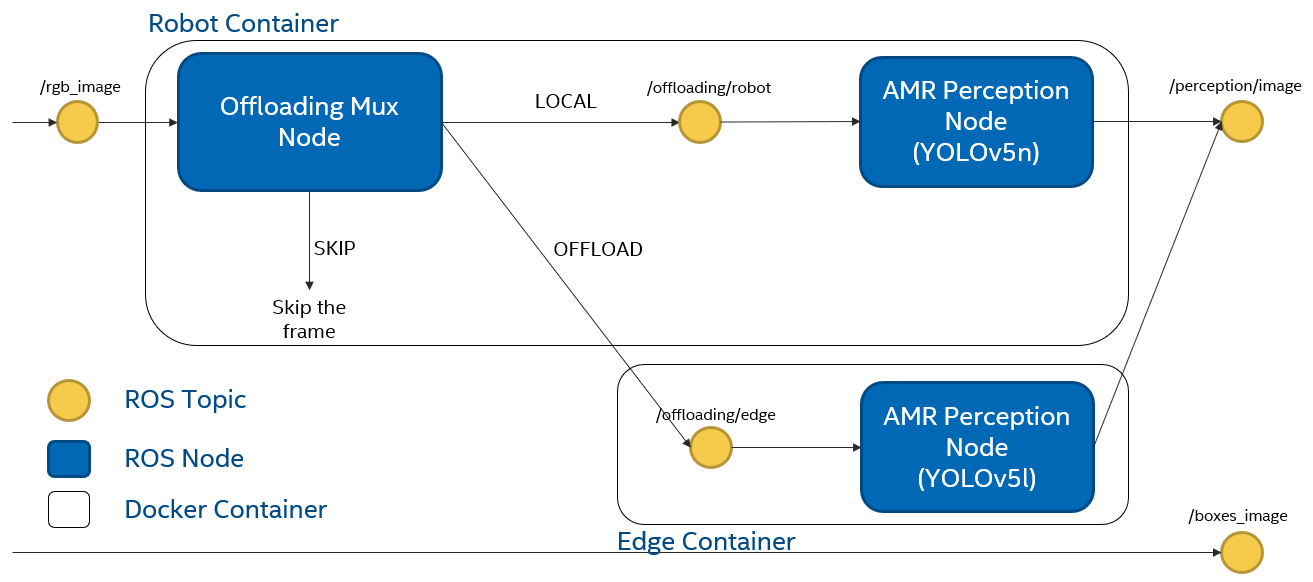
\includegraphics[width=\linewidth]{source/general_setup.png}
    \caption{Offloading framework implementation (TODO: adapt this fig)}
    \label{fig:offloading_frame_work_implementation}
\end{figure}

\subsection{Offloading Module}

% Add how is offloading module is implemented in ROS

\subsection{Perception Module}

% discuss the choice of synchronous inference and asynchronous inference. Also defend not retraining the model.

% TODO: add specifications for pytorch perception, e.g., IoU threshold etc. 

% TODO: find the quote on the edge computers
In general, an offloading task can be any computationally intensive algorithms an \gls{amr} is required to run, such as perception, navigation, \gls{slam}, path planning, etc. This thesis chooses an object detection task as an example because an object detection task can have a significant performance difference between the robot's onboard system and the edge computer, which corresponds to the usage scenario of the edge offloading. An \gls{amr} is usually equipped with a simple onboard system with only access to \gls{cpu}, while edge computers are usually cloudlets and data centers on-premise with access to \gls{gpu}. As mentioned in (TODO: add a reference here), the \glspl{amr} use primarily \glspl{dnn} to detect objects. With frameworks like PyTorch that can make use of the \gls{gpu}, the performance difference between \gls{amr}'s onboard system and the edge computer is immense. Therefore, this thesis chooses object detection as an example for offloading tasks. 

% Table for inference time on different machines
\begin{table}[htb]%
    \centering%
    \begin{tabular}{lccccc}
        \toprule
        Model &                     YOLOv5n &   YOLOv5s &   YOLOv5m &   YOLOv5l &   YOLOv5x \\
        \midrule
        Robot inference time &      50.88 ms &  115.75 ms & 240.06 ms & 464.22 ms & 821.93 ms  \\
        Edge inference time &       8.87 ms &   11.51 ms &  20.35 ms &  31.18 ms &  52.55 ms  \\
        Model size &                4 MB &      14 MB &     41 MB &     89 MB &     166 MB    \\
        \gls{map} &                 45.7\% &    56.8\% &    64.1\% &    67.3\% &    68.9\%  \\
        \bottomrule
    \end{tabular}
    \caption{Inference times of different YOLOv5 models on \gls{amr}'s onboard system and edge computer}
    \label{tab:inference_time}%
\end{table}

% TODO: better phrasing
In order to adapt to the performance difference between the \gls{amr}'s onboard system and the edge computer, the perception module should have two models available for object detection: a lightweight model that runs on the onboard system and a more complex model that runs on the edge computer. \gls{yolov5} provides a series of models with different complexities. To find appropriate models for the onboard system and the edge computer, this thesis investigates the inference times of different models on different machines, which can be taken from \cref{tab:inference_time}. To simulate the computation capability discrepancy between the two systems, this experiment uses a \gls{nuc} equipped only with an Intel(R) Core(TM) i3-8109U \gls{cpu}. On the other hand, the edge computer is equipped with an Intel(R) Core(TM) i9-7900X \gls{cpu} and a Nvidia GeForce GTX 1060 6GB \gls{gpu}. The models are deployed with \gls{pytorch} and output an array of bounding box detection. The inference time is measured between the time when the \gls{yolov5} receives the image and the time when the perception node outputs an array of bounding box detection. This includes the time for image pre-processing and the time of results post-processing. Furthermore, the image input for the offloading module has a frame rate around 25 frames per second. To achieve real-time, it is necessary that the inference time does not exceed 100 ms (\textbf{\textit{maybe phrase it better here}}). Longer inference time also causes the actual precision of the object detection to deteriorate, which will be discussed in (TODO: add a reference here). The model sizes and the \gls{map} data are taken from the documentation from \citeauthor*{Jocher2022} \cite{Jocher2022}. The \gls{map} data are evaluated on \gls{coco} val2017 \cite{Lin2014}. As a compromise between the inference time and the performance, this thesis chooses to deploy \gls{yolov5}n on the \gls{amr}'s onboard system and \gls{yolov5}l on the edge computer. 

To delimit, the object detection models in use are pre-trained and not re-trained with custom data from the simulation. This thesis intends to investigate different offloading strategies and generating custom data sets and re-training the models are laborious tasks. Therefore, a re-training of the models is beyond the scope of this thesis. \citeauthor*{Jocher2022} \cite{Jocher2022} state that the all pre-trained models are trained on \gls{coco} data-sets for 300 epochs with default settings. Moreover, this thesis only considers human obstacles, which is a detection class in \gls{coco} data sets. Therefore, the pre-trained models can provide comparability between different offloading strategies on different machines. Furthermore, re-training of the models is dependent on the quality and the size of the custom data sets. An improper re-training can introduce additional errors or over-fitting of the models and thus undermine the comparability. 

% ------------------------------------------------
\section{State Monitors}\label{sec:state_monitors}
% ------------------------------------------------

To evaluate different offloading strategies, this thesis needs to get access to the system states, such as the \gls{cpu} usage, energy consumption, and network bandwidth. Various modules are implemented to measure them. 
The measurements from these modules are recorded for evaluation and also used for dynamic strategies that make decisions based on the run-time states of the system. However, in simulation experiments, the virtualization of the \gls{amr}'s onboard system and the edge computer is realized by the \gls{docker} containers. In contrast, different physical computers are used in real-robot experiments. This difference in the system virtualization affects how the system states are measured. 

\subsection{Network}

\subsection{Onboard resources}
For simulation experiments, \gls{docker} provides the containerized system virtualization and virtual network interfaces. \citeauthor*{Ruggeri2022} \cite{Ruggeri2022} proposes that the network bandwidth in use can be measured with the network throughput. The network throughput and \gls{cpu} usage can be measured with the statistics of the \gls{docker} containers, which is a functionality provided by \gls{docker}. Alternatively, the system states of containers can be monitored using \gls{cadvisor}. For real-robot experiments, the \gls{cpu} usage and the network throughput are measured separately on different machines using \gls{psutil} tools. In the case of Intel \glspl{cpu}, the power consumption can be measured with \gls{rapl} provided by \gls{linux} kernel Power Capping Framework. The measurements of CPU usage, network throughput, and power consumption are provided by the "system status" Python package of the code base of \gls{amsrl}. \citeauthor*{Xie2021} \cite{Xie2021} propose that the execution latency of the offloading task consists of two components: the network delay and the inference time. The network delay measures the time needed for transferring the data from the offloading module to the perception module, while the inference time measures the time the perception module needs to process the inference, including the time for image pre-processing and result post-processing. The execution latency is measured with timers residing in the offloading module and the perception module. The timers record the time stamps to critical time points in the transfer and inference process and calculate the time difference. Then, the data are published to a \gls{ros} topic and can be accessed by other subscribers. 

% TODO: not sure if this paragraph is necessary
Since it is assumed that the edge computer has abundant resources, the system states of the edge computer are not measured and are not taken into consideration during the decision-making and evaluation process. Furthermore, even though this thesis only investigates the single-robot single-edge scenario, the available resources from the edge computers can be affected by numerous factors in real-world applications, such as the number of edge computers, the number of \glspl{amr}, and other processes running the edge computers. In addition, with more powerful hardware and easy access to a power supply, the edge computer consumes more energy and computation resources for the same task than the \gls{amr}'s onboard system. Therefore, it is pointless to compare the consumption of the resources between two systems with na\"{i}vet\'{e}. In contrast, the network connection between the \gls{amr} and the edge computer is fragile and prone to disturbance. Therefore, this thesis only considers the system states of the \gls{amr}'s onboard system and the network condition between the \gls{amr} and the edge computer. 
